%!TEX root = ../memoire.tex

\chapter{Un dictionnaire de patrons de régime: VerbNet}

\section{VerbNet}

Ainsi, tel que mentionné précédemment, VerbNet a été créé dans un contexte où il y avait un réel besoin pour un dictionnaire décrivant la richesse et la complexité que démontrent les verbes \citep{KipperClassBasedConstructionVerb2000}. Schuler trouvait qu'il y avait un manque de lignes directrices par rapport à l'organisation des verbes dans les dictionnaires destinés à des applications \ac{TAL}. \draft{ajouter du texte pour décrire VerbNet dans les grandes lignes et ce qu'on présentera dans la section. Levin, composantes de VN, dictionnaires concurrents, application de VN en TAL}

\subsection{Classes verbales de Levin}

Avant de parler de VerbNet, il est crucial de parler du travail qu'à fait \cite{verb-classes.levin.1993} car elle a ouvert la porte à la création de dictionnaires de verbes. Sa méthode de classification des verbes en a inspiré plusieurs dont VerbNet\cite{SchulerVerbnetBroadcoverageComprehensive2005}, et la LCS database\citep{AyanGeneratingParsingLexicon2002a}\citep{DorrUseLexicalSemantics1992}. D'ailleurs, l'architecture générale de VerbNet est basée sur ses travaux de classification des verbes.

\cite{verb-classes.levin.1993} a donc créé un dictionnaire où les verbes de la langue anglaise sont placés dans un nombre fini de classes verbales. L'appartenance à l'une d'entre elles est motivée par le partage de comportements syntaxiques communs. En observant les alternances de diathèses que démontrent les verbes, Levin remarquait que tout locuteur natif est conscient des alternances de diathèses possibles d'un verbe, et ce sans avoir de connaissances méta-linguistiques préalables. Ainsi, en se basant sur son intuition, Levin a tenté de délimiter tous les patrons de régime possibles pour les verbes de la langue anglaise. Lorsque plusieurs présentaient des caractéristiques communes sur le plan syntaxique, elle assemblait ces verbes ensemble. Le résultat de cela étant les classes verbales qu'elle posutle.

Bien que son travail s'insère dans le cadre de la syntaxe, elle supposait que les verbes qui se comportant de la même manière syntaxiquement possèdent probablement des propriétés sémantiques sous-jacentes communes. La logique de cette hypothèse étant que si deux verbes possèdent des composantes sémantiques similaires, il semble évident que cela se réflète à la surface par des comportement syntaxiques similaires. Toutefois, elle souligne que deux verbes d'apparence synonymiques peuvent très bien appartenir à deux classes différentes, tout comme deux verbes qui, en apparence, ne se ressemblent pas du tout, peuvent très bien partager des composantes sémantiques similaires.

\draft{Regrouper les verbes en classes verbales : avantage théorique et pratqiue. Théorique pcq démontre que des propriétés communces sémantiques mènent à des propriétés de surface communes aussi. Pratique pcq permet de construire un dictionnaire où les entrées lexicales ne sont pas prises individuellement, mais regroupées en classes. Cela faciliter l'entretien du dictionnaire.} Avec le système de Levin, lorsqu'on a fini de traiter une entrée verbale, on n'a pas besoin de décrire tous les patrons de régime qui lui sont associés car il ne nous reste qu'à l'ajouter à une classe déjà existante. Les auteurs de VerbNet qu'ils ont dû revisiter le classement initial de Levin puisqu'ils n'étaient pas d'accord avec le traitement de certaines entrées \citep{SchulerVerbnetBroadcoverageComprehensive2005}. 

Pour mieux comprendre le traitement des verbes à la Levin, voici un exemple tiré de la thèse de \cite{SchulerVerbnetBroadcoverageComprehensive2005} \draft{p.12-13}. On prend les verbes \lex{break} et \lex{cut}, puis on teste diverses configurations possibles pour décider s'ils appartiennent à la même classe. À prime abord, on pourrait penser que c'est le cas puisque leurs signifiés se ressemblent. \sem{Briser} et \sem{découper} partagent évidemment des composantes sémantiques car le sens d'altérer quelque chose est présent dans ces deux verbes. Cependant, le court exemple suivant nous démontre qu'ils appartiendraient à deux classes distinctes.

\ex. \label{transitive} \emph{Transitive construction}
	\a. John broke the window.
	\b. John cut the bread.
	
\ex. \label{middle} \emph{Middle construction}
	\a. Glass breaks easily.
	\b. This loaf cuts easily.
	
\ex. \label{intransitive} \emph{Intransitive construction}
	\a. The window broke.
	\b. \ungr{The bread cut.}

\ex. \label{conative} \emph{Conative construction}
	\a.\ungr{John broke at the window.}
	\b. John valiantly cut at the frozen loaf, but his knife was too dull to make a dent in it.

On voit d'abord que les constructions en \ref{transitive} et en \ref{middle} sont possibles pour ces deux verbes. Toutefois, en \ref{intransitive} et en \ref{conative}, on remarque qu'ils ne partagent pas ces cadres syntaxiques. \lex{Break} prend seulement la construction intransitive et exclut la conative, tandis que \lex{cut} prend la construction conative et exclut l'intransitive. Selon la logique de Levin, cela est dû à des différences de composantes sémantiques. Le verbe \lex{cut} décrit une série d'actions entreprises dans le but de séparer un objet en morceaux. Toutefois, il est possible de commencer à découper un objet sans que l'objet ne soit séparé. Dans ce scénario, on peut tout de même percevoir que l'objet a été découpé. En ce qui concerne \lex{break}, le changement d'état (le fait d'être séparé en morceau) est au c\oe{}ur même de l'évènement. Si on n'arrive pas au résultat final, une tentavive de briser quelque chose ne peut être perçue. 

Toutefois, nous devrons critiquer cette approche de Levin, car elle a omis de considérer un aspect important dans un traitement comme celui-ci. Dans l'exemple qu'elle nous fournit en \ref{intransitive} et en \ref{transitive}, \lex{break} n'a pas le même sens. Dans l'exemple \ref{intransitive}, on pourrait traduire le sens de \lex{break} par \sem{se briser} tandis que le sens de \lex{break} dans le contexte de l'exemple \ref{transitive} serait plutôt \sem{briser}. Cela a un impact direct sur la syntaxe, puisque le premier sens ne peut prendre qu'un seul argument, tandis que le second en prend nécessairement minimum deux. Cette lacune théorique de Levin est aussi présente dans VerbNet. Nous en discuterons plus en détails dans le chapitre \ref{eval} concernant l'évaluation de l'implémentation .

Bref, le projet de Levin a inspiré beaucoup de chercheurs, notamment l'équipe de VerbNet. C'est pourquoi ils ont repris une grande partie du travail de Levin dont l'organisation hiérarchique de VerbNet en classe et le regroupement des verbes en classes verbales. Toutefois, les auteurs de VerbNet ont retravaillé l'architecture de Levin et y ont apporté des corrections et améliorations \citep{verbnet.2006}.

\subsection {Composantes de VerbNet}  

Maintenant que nous avons présenté la contribution de Levin au développement de VerbNet, nous pouvons décrire les composantes de ce dictionnaire. Comme l'a fait Levin, il est aussi organisé en classes verbales. Chaque classe contient un ensemble de membres, une liste de rôles thématiques (accompagnés de restrictions sélectionnelles) utilisés pour décrire les arguments, puis un ensemble de cadres syntaxico-sémantiques. Chaque cadre est composé d'une brève description, suivi d'un exemple, puis d'une description syntaxique et sémantique\citep{SchulerVerbnetBroadcoverageComprehensive2005}.

\subsubsection{Classes verbales: organisation hiérarchique}

Les auteurs de VerbNet se sont fortement inspirés de Acquilex Lexical Knowledge Base \citep{CopestakeACQUILEXLKBrepresentation1992} pour l'organisation du lexique. Acquilex ordonnait l'information lexicale en hiérarchie. VerbNet a donc aussi implémenté un aspect hiérarchique à son dictionnaire en créant jusqu'à trois niveaux de profondeur pour organiser les classes verbales. 

Cela a entraîné la création des sous-classes. Celles-ci héritent de l'entièreté du contenu lexical de la classe qui la domine. Les sous-classes ont été créées pour spécifier qu'un sous-ensemble de verbes issus d'une classe mère démontrent des comportements syntaxiques différents du reste de la classe. Ceux-ci comprennent: les constructions syntaxiques, les prédicats sémantiques et les restrictions sélectionnelles sur les rôles thématiques {SchulerVerbnetBroadcoverageComprehensive2005}. Prenons un exemple tiré de VerbNet pour illustrer cette hiérarchie à plusieurs niveaux \draft{p.13 de Guidelines}

\begin{lstlisting}[language=XML, caption = Hiérarchie, label=hierarch]
<VNCLASS ID="spray-9.7">
    <SUBCLASSES>
        <VNSUBCLASS ID="spray-9.7-1">
                <VNSUBCLASS ID="spray-9.7-1-1">
        <VNSUBCLASS ID="spray-9.7-2">
            <SUBCLASSES/>
        </VNSUBCLASS>
    </SUBCLASSES>
</VNCLASS>
\end{lstlisting}

\texttt{Spray-9.7} est le nom de la classe qui englobe toutes les autres ici. À l'intérieur de celle-ci, on spécifie tous les membres appartenant à cette classe, les rôles thématiques, les cadres syntaxiques et les prédicats sémantiques. Puis \texttt{Spray-9.7-1} est une sous-classe qui hérite de l'information de sa mère, mais précise d'autres informations. \draft{Comme un sous-ensemble de verbes propres à ces comportements différents. Daniel: je ne comprends pas ce que tu veux dire ici} Puis \texttt{Spray-9.7-1-1} est une sous-classe d'une sous-classe, et ainsi de suite. Elle héritera des traits de sa classe mère ainsi que de la classe qui domine sa classe mère. Finalement \texttt{Spray-9.7-2} est la classe sœur de \texttt{Spray-9.7-1} donc, elle hérite aussi des traits de \texttt{Spray-9.7} mais ne partage pas les particularités de \texttt{Spray-9.7-1}.

Tel que démontré dans l'exemple \ref{hierarch}, les classes et sous-classes sont numérotées. Cette numérotation sert à expliciter la hiérarchie à l'intérieur d'une classe de VerbNet, mais elle sert aussi à regrouper des classes verbales en fonction de leur signifié. Cette numérotation est directement héritée du système de \cite{verb-classes.levin.1993}. Les nombres vont de 9 à 109 \draft{guidelines citation}. Le numéro associé à une classe sert à représenter le partage de caractéristiques sémantiques (et syntaxique) entre les classes qui partagent ce numéro. Par exemple, les classes signifiant \sem{mettre quelque chose} commenceront par le chiffre 9:

\FL{tu devrais peut-être te définir une macro pour avoir une typographie particulière pour les noms de classes : j'ai utilisé \texttt{}}

\begin{easylist}[itemize]
  & \texttt{put 9.1}
	& \texttt{put spatial 9.2}
	& \texttt{funnel 9.3}
	& \texttt{put direction 9.4}
	& \texttt{pour 9.5}
	& \texttt{coil 9.6}
	& \texttt{spray 9.7}
	& \texttt{fill 9.8}
	& \texttt{butter 9.9}
	& \texttt{pocket 9.10}
	
\end{easylist}

\subsubsection{Membres}
Traditionnellement, les entrées lexicales dans un dictionnaire représentent un seul et unique verbe. En ce qui concerne VerbNet, les entrées sont des classes verbales regroupant  plusieurs verbes à la fois. Cela permet à VerbNet de couvrir largement l'anglais sans recourir à une quantité excédante d'entrées. Pour garnir leur section \emph{Members}, VerbNet a puisé dans les travaux de Levin \cite{verb-classes.levin.1993},dans la base de données LCS \citep{AyanGeneratingParsingLexicon2002a} et a mené sa propre enquête pour délimiter à quelle classe verbale un verbe appartient.

Concrètement, cette information est encodée directement dans les entrées lexicales de VerbNet en XML. La figure suivante \ref{membre} démontre à quoi ressemble la section \emph{Members}. Cet exemple nous démontre que \lex{deal, lend, loan, pass, peddle} et \lex{refund} sont les membres issus de la classe \texttt{give-13.1}.

\begin{lstlisting}[language=XML, caption = Les membres d'une classe, label=membre]
<VNCLASS ID="give-13.1" xmlns:xsi="http://www.w3.org/2001/XMLSchema-instance"
 xsi:noNamespaceSchemaLocation="vn_schema-3.xsd">
    <MEMBERS>
        <MEMBER name="deal" 
				wn="deal%2:40:01 deal%2:40:02 deal%2:40:07 deal%2:40:06" 
				grouping="deal.04"/>
        <MEMBER name="lend" 
				wn="lend%2:40:00" 
				grouping="lend.02"/>
        <MEMBER name="loan" 
				wn="loan%2:40:00" 
				grouping=""/>
        <MEMBER name="pass" 
				wn="pass%2:40:00 pass%2:40:01 pass%2:40:13 pass%2:38:04" 
				grouping="pass.04"/>
        <MEMBER name="peddle" 
				wn="peddle%2:40:00" 
				grouping="peddle.01"/>
        <MEMBER name="refund" 
				wn="refund%2:40:00" 
				grouping="refund.01"/>
        <MEMBER name="render" 
				wn="render%2:40:02 render%2:40:01 render%2:40:00 render%2:40:03" 
				grouping="render.02"/>
        <!--removed "trade" from class because doesn't take "to-PP"-->
        <!--removed "volunteer "from class because doesn't fit dative or-->
        <!--PP recipient PP frames-->
    </MEMBERS>
\end{lstlisting}

\subsubsection{Rôles thématiques}
VerbNet critiquait les autres dictionnaires verbaux qui n'offraient pas de contenu sémantique \citep{SchulerVerbnetBroadcoverageComprehensive2005}. C'est pourquoi ils font la promotion de leur aspect sémantique via l'emploi de rôles thématiques. VerbNet emploie 23 rôles thématiques pour identifier les arguments sélectionnés par les verbes dans chaque cadre syntaxique. Il existe d'autres approches dont la numérotation des arguments\emph{Arg-1 Verbe Arg-2} comme on le voit dans PropBank \citep{PalmerPropositionBankAnnotated2005}, mais Schuler considérait que l'usage des rôles thématique permettait d'ajouter de l'information de nature sémantique. Effectivement, l'assignation d'un rôle thématique à un argument nous donne de l'information quant sur le type d'argument nécessaire pour un verbe donné. À la base, les rôles thématiques ont été mis de l'avant par Fillmore \cite{fillmore:case} et Jackendoff \cite{Jackendoff1972-JACSII-2}. Toutefois, VerbNet a créé sa propre banque de rôles thématiques. Beaucoup sont inspirés de Fillmore et Jackendoff, mais certains ont été créés pour VerbNet. Les auteurs de VerbNet précisent donc que la quantité des rôles thématiques et la qualité des rôles thématiques est assez arbitraire. Il n'y a pas de justification théorique derrière ce chiffre, mais c'est ce qu'ils ont convenu d'utiliser.

Voici la liste des rôles thématiques qu'ils ont choisis : \texttt{actor, agent, asset, attribute, beneficiary, cause, location, destination, source, experiencer, extent, goal, instrument, material, product, patient, predicate, recipient, stimulus, theme, time, topic}. Ces rôles ne sont pas spécifiques à des classes en particulier,\FL{évite ce genre de virgule ou tu juxtaposes deux idées pas directement liées syntaxiquement} les auteurs voulaient des rôles pouvant identifier tous les arguments possibles dans leur corpus. Donc, des rôles assez génériques pouvant se prêter à divers cadres.

%Par exemple, dans leur documentation, VerbNet offre un court exemple qui démontre l'utilité des rôles thématiques. Prenons les phrases suivantes:

%\ex. \label{semantic roles}
%	\a. Sandy shattered the glass.
%	\b. The glass shattered
	
%Dans l'exemple \ref{semantic roles}, pour la première phrase, on voit que \emph{Sandy} est le sujet du verbe et \emph{the glass} en est l'objet direct. Tandis que dans la seconde phrase, \emph{the glass} devient le sujet du verbe et il n'y a pas d'objet direct. Si on assigne un rôle d'Agent à \emph{Sandy} et un rôle de Patient à \emph{the glass}, on conserve le sens que c'est la vitre qui se casse. C'est possible grâce à l'étiquette de Patient à \emph{the glass} qui garde son rôle malgré qu'il a été promu au rang de sujet du verbe et qu'il n'y ait plus d'objet direct. C'est une manière de tenir compte de la sémantique des actants malgré les changements syntaxiques. VerbNet voulait se servir de cette théorie pour enrichir son dictionnaire.

À l'intérieur de chaque classe verbale (et sous-classe si c'est nécessaire), les rôles thématiques en jeu y sont listés dans la section \lstinline|<THEMROLES>|. Ils sont ensuite \draft{mappés} aux arguments sélectionnés dans les cadres syntaxiques et sémantiques (qu'on voit à la figure "cadres syntaxique").

\begin{lstlisting}[language=XML, caption = Les rôles thématiques] % Majuscule aux captions
    <THEMROLES>
        <THEMROLE type="Agent">
            <SELRESTRS logic="or">
                <SELRESTR Value="+" type="animate"/>
                <SELRESTR Value="+" type="organization"/>
            </SELRESTRS>
        </THEMROLE>
        <THEMROLE type="Theme">
            <SELRESTRS/>
        </THEMROLE>
        <THEMROLE type="Recipient">
            <SELRESTRS logic="or">
                <SELRESTR Value="+" type="animate"/>
                <SELRESTR Value="+" type="organization"/>
            </SELRESTRS>
        </THEMROLE>
    </THEMROLES>
\end{lstlisting}

Pour les besoins de notre travail, nous n'utilisons pas les rôles thématiques dans notre travail,\FL{formulation redondante} mais nous voulions souligner qu'ils étaient importants pour les créateurs de VerbNet. 
\draft{Voir les raisons de Melcuk p.230}

\subsubsection{Restrictions sélectionnelles}

Les restrictions sélectionnelles s'ajoutent aux rôles thématiques. Il s'agit de restrictions imposées aux rôles thématiques\FL{redondant} afin que certains types d'arguments soient sélectionnés.
Ces traits fournissent encore plus d'informations sémantiques sur l'argument. Dans l'exemple fourni ici, on remarquera que l'Agent est de type animé ou une organisation.

\begin{lstlisting}[language=Xml, caption = Les restrictions sélectionnelles]
    <THEMROLES>
        <THEMROLE type="Agent">
            <SELRESTRS logic="or">
                <SELRESTR Value="+" type="animate"/>
                <SELRESTR Value="+" type="organization"/>
            </SELRESTRS>
        </THEMROLE>
\end{lstlisting}

\subsubsection{Cadres syntaxiques}

Les cadres syntaxiques sont compris dans la section \lstinline{<FRAMES>}\FL{lstinline} de VerbNet. À l'intérieur de cette balise, on retrouve une autre balise, se nommant \emph{FRAME}, qui contient les balise \emph{SYNTAX} et \emph{SEMANTICS}. Respectivement, la première décrit un comportement syntaxique régie par la classe verbale, tandis que la deuxième décrit les prédicats sémantiques impliqués pour un tel cadre. La balise \emph{SYNTAX} nous donne une description d'une réalisation de surface d'une construction syntaxique.

Tel que mentionné plus tôt, comme le reste des informations mentionnées jusqu'à présent, les cadres syntaxiques sont partagés par l'ensemble d'une classe. Toutefois, lorsque certains cadres syntaxiques sont spécifiques à un sous-groupe, on crée une sous-classe qui aura une balise \emph{FRAMES} contenant les cadres syntaxiques propres à ce sous-groupe de verbes. Cette section nous donne de l'information de nature syntaxique. Elle explicite les liens qui unissent les rôles thématiques au verbe et l'ordre dans lequel ils peuvent apparaître en surface. Cette section est celle que nous voulions extraire pour notre travail. Nous voulons un dictionnaire qui énumère exhaustivement tous les arguments sélectionnés par des verbes. Ainsi, cette section démontre explicitement comment le verbe se combine, avec quel type d'argument, quel genre de préposition il régit.

Dans la figure ci-dessous, on voit la balise \emph{SYNTAX} qui se trouve à l'intérieur de la balise \emph{FRAME}. Puisque cette structure syntaxique est tirée de la classe \emph{ID="give-13.1"}, une réalisation de surface possible pour ce cadre serait: \emph{They lent a bicycle to me}. Dans ce contexte, \form{Paul} est l'agent, puis on a le verbe, suivi d'un thème, puis d'une préposition et finalement du récipiendaire.

\begin{lstlisting}[language=Xml, caption = cadres syntaxiques]

            <SYNTAX>
                <NP value="Agent">
                    <SYNRESTRS/>
                </NP>
                <VERB/>
                <NP value="Theme">
                    <SYNRESTRS/>
                </NP>
                <PREP value="to">
                    <SELRESTRS/>
                </PREP>
                <NP value="Recipient">
                    <SYNRESTRS/>
                </NP>
            </SYNTAX>
\end{lstlisting}

\subsubsection{Prédicats sémantiques}

En lisant la revue de littérature de VerbNet,\FL{REF?} une caractéristique distincte sur laquelle les auteurs\FL{C'est eux qui lisent?} ont misé, est l'aspect sémantique du dictionnaire. Ils contestaient le fait que beaucoup de dictionnaires faisaient un traitement syntaxique superficiel et délaissaient complètement la sémantique. C'est pourquoi ils ont développé une section sémantique. Cette section est constituée d'une suite de prédicats sémantiques. Chaque prédicat est décrit par une liste d'arguments, qui sont à leur tour décrits par deux caractéristiques: \emph{type} et \emph{value}.  Le cadre sémantique ci-dessous complète le cadre syntaxique que nous venons d'exposer. Ainsi, il s'agit de la sémantique qu'on retrouverait si on analysait une phrase comme: \emph{They lent a bicycle to me} ou \emph{They lent me a bicycle}. Ça peut décrire ces deux situations puisqu'on fait abstraction de la syntaxe et on traite uniquement les prédicats en jeu.

\begin{lstlisting}[language=Xml, caption=Les prédicats sémantiques]
<SEMANTICS>
                <PRED value="has_possession">
                    <ARGS>
                        <ARG type="Event" value="start(E)"/>
                        <ARG type="ThemRole" value="Agent"/>
                        <ARG type="ThemRole" value="Theme"/>
                    </ARGS>
                </PRED>
                <PRED value="has_possession">
                    <ARGS>
                        <ARG type="Event" value="end(E)"/>
                        <ARG type="ThemRole" value="Recipient"/>
                        <ARG type="ThemRole" value="Theme"/>
                    </ARGS>
                </PRED>
                <PRED value="transfer">
                    <ARGS>
                        <ARG type="Event" value="during(E)"/>
                        <ARG type="ThemRole" value="Theme"/>
                    </ARGS>
                </PRED>
                <PRED value="cause">
                    <ARGS>
                        <ARG type="ThemRole" value="Agent"/>
                        <ARG type="Event" value="E"/>
                    </ARGS>
                </PRED>
            </SEMANTICS>
\end{lstlisting}

Pour mieux exposer leur sémantique, nous avons fait un graphique qui exemplifie la sémantique de ce cadre.

\begin{figure}[h]
	\centering
	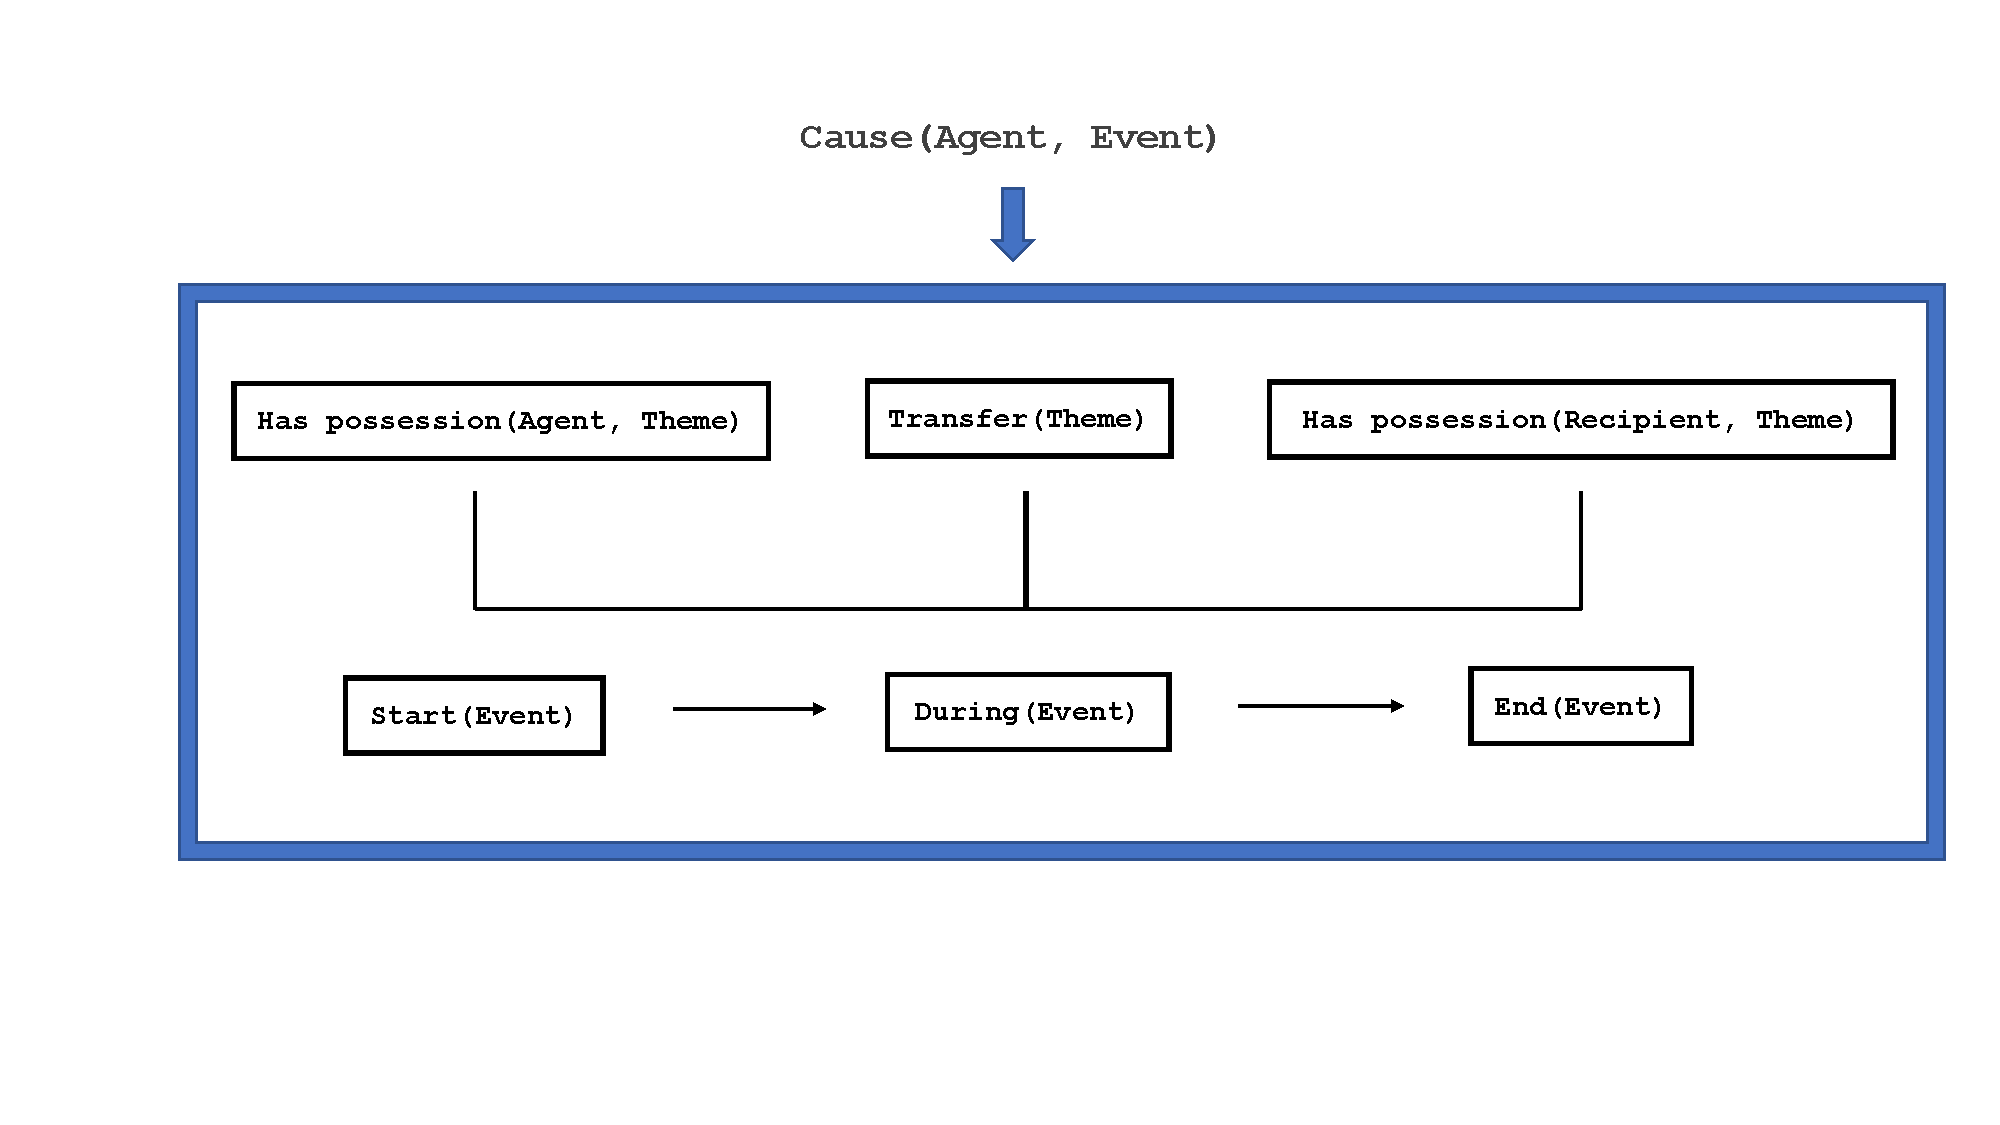
\includegraphics[width=1\textwidth, trim = {0cm 2cm 0cm 2cm},clip]{ch4/figs/semantics_give.pdf}
	\caption{prédicats sémantiques}
	\label{fig:Prédicat}
\end{figure}

\draft{Est-ce que je l'explique en détail ? Car je n'utiliserai pas du tout leur approche sémantique.}\FL{non pas la peine de trop élaborer}
%Ainsi, dans une situation où quelqu'un prête quelque chose à quelqu'un, on retrouve un sens de causation, car l'agent qui donne un objet provoque l'existence même de l'évènement en agissant. C'est pourquoi le sens de causation domine le graphique. Puis, il y a la description de l'évènement nouvellement causé. Celui est décrit à deux niveaux simultanément. Au premier niveau, on retrouve les prédicats et leurs arguments. D'abord, le premier prédicat détient la valeur 'possession' puis ses arguments sont deux rôles thématiques (l'agent et le thème). Autrement dit, quelqu'un possède un objet. En même temps, c'est le début de l'évènement.


\subsection{Dictionnaires verbaux concurrents}

Dans la section suivante, nous faisons une revue de littérature concernant les autres dictionnaires verbaux qui existent \draft{sur le marché}. \draft{Focusent généralement sur les cadres de sous-catégorisation (valence, patron de régime, structure argumentale, etc.) . Devrais-je exliquer c'est quoi ici ?}\FL{tu devrais l'expliquer au tout début: c'est le sujet de ton mémoire!}

\subsubsection{WordNet}
Wordnet\FL{REF?} est une base de données lexicales traitant les verbes, noms, adjectifs et adverbes de la langue anglaise. Cette base de données s'organise en \emph{synset}, des ensembles de synonymes. Il ne s'agit pas nécessairement de synonymes exacts, mais plutôt d'un ensemble de mots\FL{utilise la bonne terminologie: ce sont des lexies} \FL{d'une même partie du discours} unis par des traits conceptuo-sémantiques. Ces \emph{synset} sont associés à une définition et un exemple d'utilisation. Comme VerbNet, WordNet est aussi une base de données hiérarchisée. Elle est construite via des liens d'hyperonymie et d'hyponomie entre les \emph{synsets}, ce qui nous permet de naviguer dans la hiérarchie des concepts. Ainsi, tel que mentionné, les entrées lexicales dans ce système sont des synset et ceux-ci appartiennent à l'une des classes suivantes. S'il s'agit de verbes dénotant des actions ou des évènements, ils seront classés parmi: \emph{ motion, perception, contact, communication, competition, change, cognition, consumption, creation, emotion, perception, possession, bodily care and functions, social behavior and interactions}. S'il s'agit de verbes dénotant des états, on le retrouvera parmi les classes de type: \emph{resemble, belong, suffice}, ou des classes de type: \emph{want, fail, prevent, succeed}, ou de types aspectuels comme \emph{begin} \citep{Fellbaum1998}. À l'intérieur d'une entrée, on retrouve aussi des liens lexicaux: synonymes, antonymes, troponymes, implication et causation \citep{SchulerVerbnetBroadcoverageComprehensive2005}. Ce qui leur a permis de tisser une toile sémantique assez volumineuse.\FL{pas de verbe}

À la base, WordNet a été conçu comme réseau lexical, c'est pourquoi il contient peu d'information syntaxique explicite. La ressource fournit des définitions, des exemples et des \emph{synsets}, mais ne nous donne pas d'information sur la structure sémantique ou syntaxique des verbes. Elle est systématiquement implicite, contrairement à VerbNet, qui explicite cette information. Il s'agit de la raison principale qui nous a poussé à ne pas utiliser cette ressource pour créer notre dictionnaire verbal. Nous voulions une base de données explicitant très clairement les différents actants régis par un verbe, ainsi que les prépositions sélectionnnées par celui-ci. Toutefois, notre dictionnaire a la possibilité d'être aussi \draft{mappé} aux entrées de WordNet, car VerbNet a fait un \draft{mapping} entre ses entrées lexicales et celles de WordNet. Chaque verbe dans VerbNet est \draft{mappé} à un \emph{synset} verbal de WordNet, si c'est possible et qu'il y existe un équivalent \citep{SchulerVerbnetBroadcoverageComprehensive2005}.

\draft{manque les statistiques}

\subsubsection{FrameNet}

Parallèlement au projet WordNet, s'est développé FrameNet. Le projet de Berkeley FrameNet est basé sur un corpus manuellement annoté, qui contient de l'information sur les noms, adjectifs et verbes de la langue anglaise. Dans FrameNet, les unités lexicales sont décrites en termes de \emph{frame semantics}, qu'on traduirait par la sémantique des cadres.Les semantic frames sont définis comme des représentations schématiques de situations impliquant des participants , propositions et d'autres rôles conceptuels Le but de cette ressource est d'encoder la sémantique du lexique de l'anglais dans un modèle que peuvent lire les machines \citep{BakerBerkeleyFrameNetProject1998}. Ce projet couvre la sémantique des domaines suivants: santé, chance, perception, communication, transaction, temps, espace, corps , motion, étapes de la vie, contexte sociaux, émotion et cognition. Cette base de données lexicales est composée de trois modules. D'abord, un dictionnaire dont les entrées sont les unités lexicales traitées. Suivi d'un dictionnaire de \emph{frames} et complété par des exemples annotées manuellement correspondant aux \emph{frames}. Ainsi, il faut passer par le dictionnaire d'entrées lexicales, pour ensuite identifier le cadre qui lui est associé dans le dictionnaire de cadres sémantiques. Ainsi, il faut d'abord chercher dans le dictionnaire d'entrées lexicales pour ensuite trouver le ou les cadres qui lui sont associés dans le dictionnaire de cadres sémantiques. D'ailleurs, les descriptions des frames sont encodés en structures conceptuelles. Et les phrases exemples manuellement annotées sont des preuves empiriques que les \emph{frames} ont lieu d'être. Les frames décrivent la structure argumentale d'une unité lexicale. Ces arguments sont identifiés par des étiquettes similaires aux rôles thématiques. On les appelle des \emph{frame elements} et ils sont extrêmement nombreux car ils sont spécifiques aux cadrex qu'ils décrivent.En frame semantics, un frame correspond à un scénario qui implique une intéraction et des participants \citep{Shi:2005:PPT:2132047.2132058}. À noter qu'il y existe aussi une organisation hiérarchique où on a des sous-frames qui héritent de traits des frames parents. Tout comme VerbNet l'a fait avec WordNet, un mapping a été effectué entre les entrées de VerbNet et FrameNet. Cela s'est fait en deux étapes, ils ont mapper les classes de VN avec les frames de FN, puis les frames elements aux rôles thématiques \citep{Shi:2005:PPT:2132047.2132058}. Finalement, d'un point de vue pratique, FN est généralement utilisé comme \emph{semantic parser}. Des chercheurs font des parse tree syntaxique mais qui tiennent compte des participants et de leur relation avec le verbe\citep{Shi:2005:PPT:2132047.2132058}.

\draft{manque les statistiques
Expliquer pourquoi nous n'avons pas choisi FrameNet: n'explicite pas très clairement les patrons de régime. On les comprend via les phrases exemples et les frames elements, mais ce n'est pas suffisant, il y aurait beaucoup de travail à faire avant de l'implémenter dans MATE.}\FL{Marie-Claude travaille avec FrameNet, lisse bien cette section}

\subsubsection{XTAG}
Les chercheurs du projet XTAG ont construit une grammaire de la langue anglaise basé sur le formalisme de \emph{Tree Adjoining Grammar} (TAG). Cette ressource offre des descriptions syntaxiques riches des verbes en anglais. Chaque unité lexicale se fait assigner un ensemble d'arbres-TAG décrivant ses comportements syntaxiques. Les arbres reflètent la structure argumentale de ces unités lexicales. Les arbres peuvent se construire via deux opérations: substitution et adjonction. En adjoignant de nouvelles branches ou en substituant des branches, la grammaire TAG permet de rendre compte des divers phénomènes linguistiques de la langue anglaise. XTAG inclut des descriptions syntaxiques pour 33 000 items lexicaux dont 9000 verbes \citep{ResearchGroupLexicalizedTreeAdjoining2001}. XTAG organise son information syntaxique en créant des familles d'arbres. À l'intérieur de celles-ci, on distingue les arbres par des alternances syntaxiques. Ainsi, dans XTAG, Les classes verbales sont organisées de cette manière: chaque verbe dans le dictionnaire correspond à plusieurs familles d'arbres et chaque famille regorge d'arbres individuels issus de différentes transformation syntaxiques de surface pour une même structure argumentale canonique. Ainsi, on n'a pas à lister tous les arbres individuels possibles correspondant à un verbe, car celui-ci se fait assigner des familles d'arbres \citep{DoranXTAGSystemWide1994}.

Finalement, comme avec WordNet et FrameNet, Les auteurs de VerbNet ont aussi mappé leurs cadres syntaxiques aux arbres de XTAG \citep{W04-3326}.
D'ailleurs, cela leur a permis de couvrir des descriptions syntaxiques qu'ils n'avaient pas répertoriés. VerbNet couvre surtout la voix déclarative, tandis que XTAG explore toutes les transformations possibles de voix. Cependant, XTAG ne fait pas de distinctions pour les différents sens des verbes et il s'agit là d'une composante cruciale à la construction d'un bon dictionnaire en GAT. C'est pourquoi nous n'avons pas opté pour ce dictionnaire. De plus, le formalisme dans lequel les arbres sont encodés ne s'exporte pas facilement dans un format réutilisable en TST.

\draft{Si j'ai le temps, traiter un peu de G-TAG dans cette partie}

\subsubsection{Lexical conceptual structures-LCS}
La base de données LCS de Dorr s'est construite à partir des théories de sémantique lexicale de Jackendoff. Celui-ci argumente en faveur d'une approche de décomposition sémantique des verbes. Ceux-ci sont décrits en termes de leur structure conceptuelle lexicale\citep{DorrUseLexicalSemantics1992}. Une structure LCS est un graphe, il s'agit d'une représentation sémantique du lexique. Dans ce système, la structure syntaxique découle des primitifs sémantiques. Un graphe LCS est une représentation sémantique où il y a des noeuds dont une racine. Chaque noeud a des spécifications avec des types d'information comme: type, primitif et champ. Type ; event, state, path, manner,etc. Puis après avoir spécifier le type, on spécifie le primitif sémantique du verbe (être, aller, rester,etc.)  et les champs sont des traits qui agissent comme des restrictions sur les noeuds.Ces structures sont des représentations hiérarchiques non-linéaire composées d'une tête logique (la racine du graphe), d'un sujet logique (un seul) , d'arguments logiques et de modificateurs logiques. En ce qui concerne le traitement des verbes, la racine du graphe sera un verbe et les sujets/arguments logiques seront les participants sélectionnés par le verbe. Concrètement, ce qui décrit la sémantique des graphes est une combinaison de constituents et primitifs conceptuels et de champs sémantiques. D'abord, les constituents conceptuels appartiennent à un ensemble de catégories: chose, évènement, état, lieu, chemin, propriété, but, manière, montant, temps. Ensuite, les champs sémantiques sont des traits qui agissent comme des restrictions sélectionnelles(ex: +temp, +loc, +poss). Finalement, les primitifs conceptuels: ÊTRE, ALLER, RESTER , CAUSER, INCHOATIF, EXTENSION. Une décomposition sémantique des verbes en termes de structures lexicales conceptuelles explique leur propriété syntaxiques. Tel que Levin l'avait perçu, les propriétés sémantiques des verbes influenceront leur comportements syntaxiques. À l'intérieur de ce cadre théorique, on pense que les verbes avec des LCS similaires partagent aussi des comportement syntaxiques comme des alternances de diathèses. Ils utilisent aussi des rôles thématiques pour montrer la structure argumentale. La base de données de Dorr prend aussi la hiérarchie et se base sur les classes de Levin pour structurer son information. Dans cette base de données, les verbes sont aussi rassemblés en classes verbales. Ce qui unit les membres à une classe verbale est le partage d'une structure LCS commune. Ainsi, tous les membres d'une classe partage la même structure sémantique, mais le contenu sémantique selon chaque verbe pour satisfaire les contraintes lexicales de ceux-ci \citep{TraumGenerationLexicalConceptual2000}. 

Nous n'avons pas pris cette ressource car nos représentations sémantiques opèrent déjà la même fonction que ces graphes LCS. De plus, le caractère syntaxique de ce système ne fournit pas du tout ce que nous cherchions. Nous voulons un dictionnaire qui énumère les différents patrons de régime possibles pour un verbe donné. Toutefois, ce système a été utilisé de la même manière que nous générons du texte automatiquement en différentes langues. Cette base de données lexicales a été utilisée pour faire de la traduction automatique \citep{DorrUseLexicalSemantics1992}. Cela a été fait dans le cadre du projet UNITRAN qui traite:l'espagnol, l'anglais et l'allemand. À l'aide de représentation basées sur la LCS , ils pouvaient générer des traductions équivalentes entre les langues à partir d'une même représentation. Par la suite, les dictionnaires se chargent des spécificités de chaque langues. Notre système GenDR fonctionne aussi de cette manière.

manque les statistiques

\subsubsection{Comlex}
Comlex est une base de données lexicales développée pour l'anglais à NYU. C'est une ressource syntaxique riche, mais dont il faut débourser pour s'en servir. Les auteurs de ce système voulait  créer un dictionnaire syntaxique sur les verbes de l'anglais à des fins computationelles \citep{Grishman:1994:CSB:991886.991931}. Ils ont opté pour un système qui se voulait le plus neutre du point de vue de la théorie afin qu'il puisse être utilisé dans divers cadres de recherche. Ce dictionnaire ne traite pas uniquement que les verbes, mais c'est la partie qui nous intéresse. En ce qui concerne ceux-ci, le système décrit pour chaque verbe les compléments possibles qu'il pourrait sélectionner ainsi que les spécificités propres à certaines constructions (choix d'une préposition,etc.) Les entrées lexicales ont été manuellement ajoutées car ils ne pensaient pas que des méthodes automatiques pouvait bien rendre compte des verbes moins fréquents, et ils voulaient que leurs entrées sois dépourvues d'erreurs. Contient des descriptions syntaxiques pour 6000 verbes. 

Nous n'avons pas pris ce système car, d'abord il faut payer la license, puis nous avions lu l'évaluation que VerbNet avait menée et il en ressortait que Comlex ne distingue pas les  différents sens des verbes. Ce qui est problématique si on veut générer la phrase la plus correcte possible.

\subsubsection{A large SCF lexicon for NLP apps: Valex}
 
Valex est un projet de Korhonen, il s'agit d'un dictionnaire de cadre de sous-catégorisation (SCF) de l'anglais \citep{Korhonenlargesubcategorizationlexicon2006}. Elle a bâti son dictionnaire via des méthodes d'acquition automatiques. L'auteure vante les mérites d'une acquisition automatique et se défend en stipulant que les dictionnaires bâtis manuellement comportent naturellement plus d'erreurs. Elle pense aussi qu'ils sont plus coûteux en termes de temps et de ressource, car il faut les entretenir et les enrichir. Finalement, elle ajoute que les dictionnaires manuellement acquis comportent une faille cruciale, il leur manque de l'information statistique. Par exemple, quel cadre de sous-catégorisation est le plus utilisé pour un verbe donné et les SCF les moins fréquents.  Puisque de nombreuses applications TAL fonctionnent avec des méthodes probabilistes, la présence d'information statistique est cruciale à leur bon fonctionnement.  

Dans son article, elle explique qu'elle a utilisé le système d'acquisition de Briscoe et Caroll \citep{BriscoeSecondReleaseRASP2006} qui se base sur la méthode RASP. À partir de textes non-annotés, les SCF sont extraits grâce au système RASP. Ainsi, les données brutes provenant des corpus sont d'abord tokénisées, étiquettées, lématisées puis parsées utilisant RASP. Puis les SCF sont extraits des phrases parsées. Ainsi, chaque entrée lexicale est une combinaison d'un verbe et d'un SCF ce qui résulte en un dictionnaire de base. Finalement, il est filtré car, puisque c'est une méthode automatique, le système déduit des SCF qui n'en sont pas. Il faut donc les retirer du dictionnaire. D'ailleurs, ces systèmes se retrouvent avec des problèmes de rappel. Certains SCF ne seront pas extraits puisque le système ne les reconnaîtra pas comme des SCF. Ils utilisent des dictionnaires construits manuellement pour trouver ces SCF manquants.

Dans Valex, une entrée lexicale comprend entre autre: la combinaison d'un verbe et d'un SCF, la syntaxe des arguments, la fréquence d'utilisation du SCF. Bien que ce système aurait été potentiellement bon, nous avons préféré nous tourner vers VerbNet. D'abord, ce dictionnaire ne différencie pas les sens des verbes, de plus, l'architecture du logicielle ne nous permet pas de tirer parti du principe d'héritage des traits. Contrairement à VerbNet qui le permet, d'autant plus que ça permet de réduire la quantité d'information dans notre dictionnaire. Finalement, comme notre système fonctionne avec des règles de grammaire et que ce n'est pas un générateur de texte basé sur des méthodes stochastiques, l'apport d'informations statistiques que Valex offre ne nous était pas utile pour l'instant.

statistiques: coverage

\subsubsection{LexSchem}
LexSchem est un dictionnaire de verbe pour le français créé par Messiant. Il jusitifiait la valeur de son projet en disant que  que l'information la plus utile qu'un dictionnaire peut offrir sont les cadres de sous-catégorisation des verbes \citep{MESSIANT08.142}. Ces \emph{subcategorization frame} (SCF) capturent, au niveau syntaxique, les différentes combinaisons d'arguments qu'un prédicat lie. Messiant ajoute que comme les verbes sont au centre des énoncés, un dictionnaire qui se concentre sur les cadres de sous-catégorisation peut être très bénéfiques à des applications TAL.  Nous avons vu jusqu'à maintenant qu'ils peuvent être utilisés pour le parsing et la traduction automatique par exemple. Toutefois, suivant les pas de Korhonen \citep{Korhonenlargesubcategorizationlexicon2006}, Messiant a bâti un dictionnaire de SCF pour le français via une acquisition automatique. Il se justifie en disant que cette technique a déjà fait ses preuves dans des applications réelles malgré le fait qu'elle n'est pas aussi précise et détaillée qu'une approche manuelle. Mais elle est beaucoup moins coûteuse en termes de temps et de ressource. De plus, une approche automatisée permet d'extraire de l'information qui pourrait s'avérer très utile pour des applications TAL. Notamment, les statistiques et la fréquence d'utilisation d'un SCF.  Son dictionnaire a été acquis à partir de corpus non-annoté. Par la suite,les SCF acquis automatiquement sont incorporés dans lexSchem. Voici la démarche qu'il utilisa, d'abord ils prennent des données brutes, puis il étiquette et lemmatise les mots  pour ensuite parser le tout. Après il ne reste qu'à en extraire les SCF. Dans LexSchem, Les entrées lexicales sont composées essentiellement de: L'unité lexicale, ses cadres de sous-catégorisation et des phrases exemples tirées de corpus ainsi que la fréquence d'utilisation du SCF.

Ce que nous retenons de ce système, c'est qu'il pourrait être utile dans un avenir où nous voulions extraire VerbeNet qui est une version francophone de VerbNet. Nous pourrions ainsi complémenter la ressource francophone par une autre ressource franchophone. De plus, tel que VerbNet l'a fait, LexSchem construit ses entrées lexicales en misant sur les cadres de sous-catégorisation. Nous pensons aussi qu'un dictionnaire verbal en TAL devrait surtout incorporer ces données, ce qui nous intéresse sont les cadres de sous-catégorisation, car ceux-ci sont la partie la plus dure à traiter en TAL.

statistiques:

\subsubsection{VDE-Valency dictionary of English}
Le VDE est un dictionnaire de valence tout comme les dictionnaires précédents qui liste la manière dont un verbe peut se combiner avec ses arguments \citep{HerbstValencyDictionaryEnglish2004}. Le VDE contient les valences de 511 verbes (il traite aussi les noms et les adjectifs). Dans ce dictionnaire, chaque entrée décrit une valence possible pour un verbe accompagné d'un exemple provenant de la \emph{Bank of English}. Lors de sa création, le VDE n'était pas destiné à des applications TAL, mais les auteurs se sont rapidement rendus compte que ça pourrait intéresser des linguistes computationnels. Ainsi est né le \emph{Erlangen Valency Pattern Bank} \citep{faucris.1039365}, un outil de TAL qui liste les patrons de valence identifié par le VDE.  Dans le VDE, les 511 verbes qui y figurent ont été choisis sur la base qu'ils sont fréquents dans la langue anglaise, qu'ils démontrent des propriétés complexes et qu'ils sont utiles pour des apprenants de l'anglais. Les patrons de valence qu'on retrouve dans le VDE proviennent d'une étude de corpus fait sur le COBUILD. Les patrons y sont décrits en termes de syntaxe de surface.  Leur dictionnaire est réparti en deux où d'un côté on a la liste des 511 verbes et les patrons de valence leur étant associés, puis dans un autre dictionnaire les patrons de valence de la langue anglaise. Il s'agit aussi d'un système qui distingue les différents sens que peuvent prendre les verbes. 

Bref, il s'agit d'un dictionnaire qui couvre de verbes, mais les plus fréquents. Toutefois, il s'agit d'un travail manuel, donc on s'attend à ce qu'il ne comporte pas beaucoup d'erreurs, et on pourrait ainsi en extraire une partie pour complémenter le dictionnaire de VerbNet si tel est le besoin.

%Thomas Herbst and Peter Uhrig. 2009. Erlangen Valency Pattern Bank – a corpus-based research tool for work on valency and argument structure constructions. Website. http://www.patternbank.uni-erlangen.de

\subsubsection{Dicovalence}
Le Dicovalence est un dictionnaire de valence pour la langue française. Une entrée lexicale dans ce dictionnaire correspond à la combinaison d'un verbe, d'un cadre valenciel et d'un exemple. Comme il y a 3700 verbes traités et que la plupart des verbes comptent plus d'un cadre valenciel, il y a plus de 8000 entrées lexicales dans ce dictionnaire. Les informations à l'intérieur des cadres valenciels sont décrites par l'approche pronominale en syntaxe \citep{11403/dicovalence/v1}.\FL{check la référence bib} Dans leur système, ce que plusieurs appellent des participants, des actants ou des arguments, sont appelés des paradigmes. Le Dicovalence a aussi été créé dans une optique de TAL et d'enseignement de la langue. Contrairement à des systèmes comme FrameNet, ou VerbNet, ils identifient leurs arguments en les numérotant. Le paradigme p0 étant souvent le sujet, le p1 étant l'objet direct, le p2 étant l'objet indirect et tous les autres étant des obliques. Ce dictionnaire contient beaucoup d'information utile autre que les cadres valenciels. Il y a : des phrases exemples, des traductions du verbe en anglais et en allemand, des restrictions sélectionnelles sur les paradigmes, le type d'auxiliaire (avoir/être) et les constructions passives.

Nous n'utiliserons pas ce système puisque nous traitons l'anglais, mais le survol de ce système nous confirme que VerbNet était un bon choix, car les entrées importantes sont souvent les mêmes. Les cadres syntaxiques, les phrases exemples. Toutefois, nous pourrions nous en servir pour compléter l'implémentation de VerbeNet français dans notre système pour une génération multilingue.

%https://repository.ortolang.fr/api/content/dicovalence/1/documentation/DicovalenceManuel_v20_100625.pdf
%Karel van den Eynde and Piet Mertens. 2006. Le dictionnaire de valence DICOVALENCE: manuel d’utilisation. http://bach.arts.kuleuven.be/dicovalence/manuel 061117.pdf.

\subsection {Utilisation de VerbNet dans des applications TAL}

VerbNet a été utilisé dans un grand nombre de travaux de recherche. Nous en mentionnons ici quelques-uns.

\subsubsection{Construction de graphes conceptuels}
\citep{HensmanAutomaticallyBuildingConceptual2004}\FL{intégrer les REF au texte}
Les graphes conceptuels servent à représenter le sens d'un énoncé. Dans une recherche, ils se sont servis des informations lexicales de VerbNet pour créer des graphes automatiquement. Ainsi, ils prennent des documents provenant de corpus, ils en extraient les phrases, ils les parsent syntaxiquement, puis les matche à un patron correspondant dans VerbNet. Après avoir un patron correspondant, la phrase est maintenant dotée de toutes les informations lexicales contenues dans les entrées de VerbNet et la création du graphe conceptuelle se fait automatiquement. Ces graphes sont ensuite ajoutés dans une base de données et ils facilient l'information retrieval.

\subsubsection{Parsing sémantique}
\citep{Shi:2005:PPT:2132047.2132058}
Dans ce projet, VerbNet est combiné à FrameNet et WordNet pour faire du semantic parsing. La force de VerbNet dans ce projet est son exhaustivité des différents patrons de régime de l'anglais, et les rôles sémantiques qui sont liés aux verbes. Ils suggèrent que l'utilité de VerbNet provient aussi de sa couverture de l'anglais et des patrons de régime possible est extrêment riche et donc cruciale pour ce genre d'opération. Le but d'un semantic parser est d'analyser le sens de la structure d'une phrase. Donc, via les ressources dont VerbNet, lorsqu'il parse un texte non annoté, le parseur cherche des patrons similaires à ceux se trouvant dans les bases de données lexicales pour ensuite étiquetté les phrases et en faire sortir la structure syntaxique et les caractérisitques sémantiques via les rôles thématiques.

\subsubsection{Un système de questions-réponses}
\citep{DBLP:conf/nlpke/WenJH08}
Pour un bon système de question-réponse, la précision de la réponse est cruciale. De parvenir à un haut niveau de précision pour une réponse, ils proposent un système de question-réponse reposant sur VerbNet. Leur système extait les informations syntaxiques et sémantiques des questions puis à partir du web formule des réponses candidates en fonction des informations extraites de la questions , puis VerbNet est appliqué dans leur système pour détecter les cadres syntaxiques des verbes dans les questions et dans les réponses candidates afin d'obtenir les informations syntaxiques et sémantiques. Puis, leur système choisi la phrase candidate répondant le mieux à la question et tenant compte de la structure sémantique et syntaxique de la question.

\subsubsection{A supervised algorithm for verb desambiguasation into VerbNet classes}
\citep{AbendSupervisedAlgorithmVerb2008}
Ils ont développé un modèle d'apprentissage supervisé pour mapper des lexèmes à des classes de VN. Comme la polysémie est un enjeu majeur en TAL, leur travail consistait à analyser un texte et lorsqu'il trouve un verbe, il doit l'associer à la bonne classe, en fonction des informations lexicales qu'on retrouve dans la classe. Développer ce genre d'outil en TAL est très important car, les machines ne voient les verbes que comme des chaînes de caractères dépourvues de sens. Le contexte d'utilisation d'un verbe nous permet de savoir à quelle classe VN il est présentement utilisé (comme bcp de verbes s'emploient avec des classes différentes selon le contexte). EN moyenne un verbe appartient à 2.5 classes différentes.

\subsubsection{VerbNet class assignment as a wsd task}
\citep{BrownVerbNetClassAssignment2011}
Des représentations verbales riches sont cruciales en NLP pour un parsing sémantique profond. Utiliser un lexicon déjà annoté à plusieurs niveaux peut être très utile pour ce genre de tâches. par exemeple la désambiguisation en serait très profitable. Leur classifieur sémantique s'apparente beaucoup à celui de Abbend \citep{AbendSupervisedAlgorithmVerb2008}.

\subsection{Synthèse}

Nous avons choisi VerbNet car c'est une ressource qui s'est distinguée de ses concurrentes. D'abord, par son imposante couverture de la langue anglaise \draft{(statistiques)}. Ensuite, par son architecture interne héritée de Levin et améliorée. Le regroupement en classes verbales facilite énormément le travail, et le découpage hiérarchique suivi des mécanismes d'héritage en font un outil très performant et précis, sans être encombrant et facilement repérable. Les verbes sont aussi classés dans plusieurs classes verbales, donc ils sont partiellement désambigguisés, ce qui est extrêmement utile, car on veut être le plus précis possible en NLG. De plus, les descriptions syntaxiques encodées en XML sont facilement exportable et maléable dans un format qui nous convenait, par le fait même, le traitement en Python devenait très accessible puisque NLTK avait déjà fait un pré-traitement de VerbNet, ainsi il existait des modules dont nous pouvions nous inspirer pour extraire l'information dans les balises de VerbNet. Un autre point important est qu'il existe beaucoup de ressources linguistiques à la VerbNet dans d'autres langues que l'anglais, dont le (mettre les citations de tous les verbnet étrangers) français, le portugais, l'italien, l'estonien, l'espagnol, le catalan, le tchèque. Finalement, puisque notre système GenDR se veut un générateur multilingue dans sa première version, c'est un premier pas pour facilement implémenter d'autres langues à notre système puisque nous avons déjà des scripts une architecture prête pour acceuillir des ressources lexicales similaires. 

De plus, dans la section précédente, on montre qu'il est utilisé pour des applications de TAL diverses, mais on a aussi trouvé des systèmes récents qui utilisaient VerbNet pour faire de la NLG. Des chercheurs ont extrait le mapping qui avait été fait entre XTAG-VerbNet afin de donner une couverture imposante de l'anglais pour l'interface sémantique-syntaxe de son générateur. Ils se sont surtout servis de VerbNet pour créer leur grammaire. Leur projet s'appelle S-STRUCT \citep{PfeilAlgorithmsResourcesScalable2016}, un générateur de texte automatique dont on a ajouté un module d'apprentissage machine pour la partie \emph{discourse planning}. Ainsi, en améliorant la partie discourse planning avec du machine learning, le système apprend à générer les phrases dans un ordre statistiquement plus logique.

D'un autre côté, Wanner et Mille ont publié un court article expliquant qu'ils prévoyaient utiliser VerbNet comme base de données lexicales car ils avaient besoin d'une ressource lexicale riche dans le cadre de génération automatique de texte \citep{MilleLargeCoverageDetailed2015}. De telles ressources sont importantes pour la couverture et qualité des en GAT. Ils mentionnent que des réaliseurs classiques comme KPML, surge, et REALpro \FL{citations} nécessitaient un enrichissement lexical pour être encore plus performant. Car, pour arriver à une structure syntaxique de surface, où tous les unités lexicales sont réalisées, il faut qu'un système de GAT possède des ressources lexicales capables de générer tous les actants d'un verbe en fonction des restrictions possibles et des bonnes prépositions, il faut que la génération soit impeccable aussi. Ces informations se retrouvent dans des dictionnaires de cadres de sous-catégorisation tel que ceux mentionnés plus haut. En anglais, VerbNet rempli très bien les caractéristiques recherchées pour des dictionnaires lexicaux car c'est un lexicon à grande surface qui couvre une grande partie de la grammaire anglaise et détaille avec précisions les patrons de régime possibles, ainsi que beaucoup d'autres informations. Toutefois, ils précisent quelque chose qui est très vrai, VerbNet est principalement utilisé pour des tâches comme semantic role labelling, information retrieval. En résumé, les ressources lexicales éxistantes sur le marché sont incomplètes et difficile à implémenter pour la NLG. Ce qui a découlé de ce travail est Forge \citep{DBLP:conf/semeval/MilleCBW17}, un générateur de texte automatique. Toutefois, ils n'ont pas utilisé VerbNet dans leur système, tel que nous l'avons vu dans la section précédente. Ce qui démontre l'importance de ce travail car nous avons décidé d'utiliser VerbNet en tant que ressource lexicale pour faire la tâche qu'ils avaient entamés, mais sur laquelle ils n'ont pas publié de résultats.
